\documentclass[a4paper, 11pt]{article}
\usepackage{graphicx} 
\usepackage[utf8]{inputenc}
\usepackage[T1]{fontenc} 
\usepackage[margin = 1in]{geometry}
\usepackage{amsmath}
\usepackage{xcolor}
\usepackage{enumitem}
\usepackage{soul}
\usepackage{setspace}
\usepackage{hyperref}
\usepackage{mathpazo}
\usepackage{booktabs}
\usepackage{listings}
\usepackage{caption}
\usepackage{float}
\usepackage{matlab-prettifier}
\usepackage{fancyhdr}

\pagestyle{fancy}
\fancyhf{}
\rhead{Student ID: 230302279}
\lhead{Sanjin Ruzic}
\title{Project Taste: Octave Coffee Machine Simulator}
\author{Sanjin Ruzic}
\date{January 3, 2024}

\hypersetup {
colorlinks = false,
filecolor = blue,
citecolor = black,
linkcolor = blue,
urlcolor = blue
}

\makeatletter         
\def\@maketitle{
\raggedright
\begin{center}

\includegraphics{./Images/IUS_Logo}
\vspace{15mm}
\end{center}
\begin{center}
{\Huge \@title }\\[4ex] 
{\Large \@author}\\[4ex] 
\@date\\[8ex]
\end{center}}
\makeatother

\begin{document}

\maketitle
\vspace{5mm}
\newpage

\tableofcontents
\newpage

\section{Introduction}
\noindent This is a comprehensive documentation and guide for Taste, a project I have been developing in GNU Octave, tool best known for its numerical computation capabilities, for my final ENS101 (Introduction to Engineering) project assignment. The cornerstone of Taste is its friendly graphical user interface (GUI), which faithfully emulates the principle of work and characteristics of coffee vending machines in the real world. Not only does it enable you to select from a wide variety of coffee types, but it also offers the customization of your selection to some degree (it is worth noting that it is purely cosmetic and does not affect the brewing process in any way). An added benefit is that you are free to tailor your own experience according to your wishes by specifying the strength of the coffee, quantity of sugar and even simulate actions such as inserting coins into the machine slot, taking change and collecting dispensed coffee.
\vspace{5mm}

\noindent In addition to replicating a realistic physical interaction scenario, Taste utilizes underlying logic fairly identical to coffee machines in the real world, which can be observed with how it handles crucial resources such as the water level, amount of coffee beans and machine money balance, alerting the user in the event of any one's depletion unless refilled by the operator. A deeper examination may lead to the acknowledgement that my project intends to explore a more practical application of key engineering principles taught during the ENS101 course.
\vspace{5mm}

\noindent The aim of this documentation is to provide a detailed overview of the design features of the project, explaining the UI components it consists of and their usefulness in a broader sense. I will also be discussing the steps I have taken in the GUI creation so that it may serve as a valuable insight into the development process and capture the full picture of my approach. Lastly, it will delve deeper into the intricacies of the functional logic responsible for the coffee machine's key operations and interactions with the user.

\section{Usage Manual}

\noindent Using the Taste coffee machine GUI is fairly straightforward. Here are the steps:

\begin{enumerate}
\item \textbf{Start the Program:}
Open the file \texttt{coffeeVendingMachine.m} in GNU Octave and run the script. After you have done this you should see the GUI window appear on your screen.
\vspace{3mm} 
\begin{figure}[H]
\centering
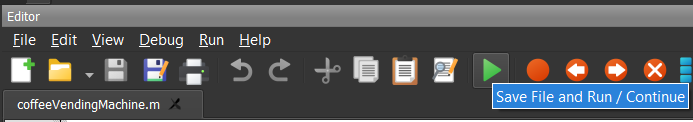
\includegraphics{Images/Figure2.1.PNG}
\caption*{\textbf{Figure 2.1} Running the script file in GNU Octave} 
\end{figure}
\vspace{5mm} 

\item \textbf{Select Coffee:}
On the GUI, you will be presented with several options for coffee types. Click on the \texttt{Select} on the panel of the coffee type that you want.
\vspace{3mm} 
\begin{figure}[H]
\centering
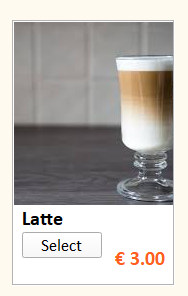
\includegraphics{Images/Figure2.2.PNG}
\caption*{\textbf{Figure 2.2} Selecting a coffee} 
\end{figure}
\vspace{5mm} 

\item \textbf{Customize Your Coffee:}
Once you have made your selection, a mini window will appear displaying more details about the coffee you have chosen. You may also customize your coffee according to your preference by selecting the coffee strength and sugar level buttons, one from each group at most.
\vspace{3mm} 
\begin{figure}[H]
\centering
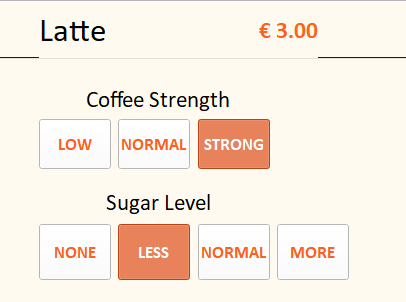
\includegraphics{Images/Figure2.3.PNG}
\caption*{\textbf{Figure 2.3} Coffee customization options} 
\end{figure}
\vspace{5mm} 

\item \textbf{Insert Money:}
You may view the price of the coffee in the same coffee details window, not only on the main panel. Hover over the \texttt{Actions} menu bar and insert the required amount with the options provided (euros are the only available currency). The GUI will track the total amount of money you inserted and be updated accordingly for each interaction.
\vspace{3mm} 
\begin{figure}[H]
\centering
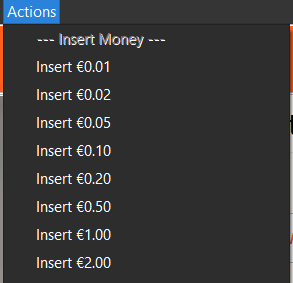
\includegraphics{Images/Figure2.4.PNG}
\caption*{\textbf{Figure 2.4} Inserting coins into the machine} 
\end{figure}
\vspace{5mm} 

\item \textbf{Collect Change:}
If you inserted more money than the coffee cost, there will be change that you have to collect before the machine can begin brewing your coffee, which is deducted from the machine's money balance. Even if the change is zero, you must press \texttt{Collect Change} in the \texttt{Actions} menu bar in order for the machine to proceed to the brewing stage.
\vspace{3mm} 
\begin{figure}[H]
\centering
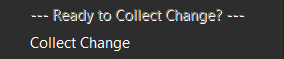
\includegraphics{Images/Figure2.5.PNG}
\caption*{\textbf{Figure 2.5} Taking the change} 
\end{figure}
\vspace{4mm} 

\item \textbf{Collect Coffee:}
Be patient while the machine is making your coffee. The prompt will inform you when it is finished and instruct you to collect the dispensed coffee. To do this, simply go to the \texttt{Actions} menu bar and press \texttt{Collect Coffee}. And just like that, you are done! The mini window automatically closes after a few seconds of inactivity and you may again repeat the process of ordering coffee by following these steps.
\vspace{3mm} 
\begin{figure}[H]
\centering
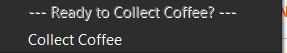
\includegraphics{Images/Figure2.6.PNG}
\caption*{\textbf{Figure 2.6} Collecting the coffee} 
\end{figure}
\vspace{4mm} 
\end{enumerate}

\section{Design Overview}
In this section, I will review the architectural aspects of the GUI. This includes GUI initialization, creation and organization of UI panels and elements, as well as the addition of a menu bar for user actions.
\subsection{Initializing the GUI}
\begin{lstlisting}[style=Matlab-editor, numbers = left, frame = single]
% Get screen size and calculate figure position
screenSize = get(0, 'screensize');
figureSize = [1000, 700];
mainFramePos = [(screenSize(3) - figureSize(1))/2, (screenSize(4) - figureSize(2))/2, figureSize(1), figureSize(2)];

% Create GUI frames
mainFrame = figure('name', 'Coffee Vending Machine Simulation', 
'NumberTitle', 'off', 
'toolbar', 'none', 
'resize', 'off', 
'position', mainFramePos, 
'visible', 'on');
mainFrame = gcf;
titleFrame = uipanel('parent', mainFrame, 
'backgroundcolor', titleBackgroundColor, 
'position', [0 0.9 1 0.1]);
coffeeSelectionFrame = uipanel('parent', mainFrame, 
'backgroundcolor', backgroundColor, 
'position', [0 0 1 0.9]);

% Text elements for title and clock
titleText = uicontrol('parent', titleFrame, 
'units', 'normalized', 
'style', 'text', 
'string', 'taste', 
'fontsize', 23, 
'fontname', 'Georgia', 
'backgroundcolor', titleBackgroundColor, 
'foregroundcolor', titleTextColor, 
'position', [0.25 0 0.5 1], 
'horizontalalignment', 'center', 
'fontweight', 'bold');
clockText = uicontrol('parent', titleFrame, 
'units', 'normalized', 
'style', 'text', 
'string', datestr(now, 'HH:MM'), 
'fontsize', 16, 
'fontname', 'Calibri', 
'backgroundcolor', titleBackgroundColor, 
'foregroundcolor', titleTextColor, 
'position', [0.8 0 0.25 1], 
'horizontalalignment', 'center', 
'fontweight', 'bold');
\end{lstlisting}
\vspace{5mm}
\noindent The purpose of the code block above is to initialize the GUI for the coffee machine simulator. First, it retrieves the screen size and defines the figure to be 1000 pixels wide and 700 pixels tall so that it may calculate the position of the main frame (GUI window), placing it at the center of the screen.
\vspace{5mm}
\newpage
\noindent By using the \textbf{figure} function, I am able to create a new figure window with the properties specified, meaning it will be visible, but will not have a toolbar or a number title, nor will it be resizable. Two panels, \texttt{titleFrame} and \texttt{coffeeSelectionFrame} are then created within the main frame with the \textbf{uipanel} function, which, similar to before, generate two panel objects parented to the main frame with the given properties. 

\vspace{5mm}
\noindent Finally, I create text elements parented to the title frame with the \textbf{uicontrol} function so that I may incorporate interactive controls, in this case two static controls that only display text in a string, namely the string \texttt{"taste"} and current time in the \texttt{HH:MM} format.

\subsection{Setting up the coffee selection panel}
\begin{lstlisting}[style=Matlab-editor, numbers = left, frame = single]
% Spacing and panel dimensions for coffee panels
spacing = 0.03;
panelWidth = (1 - 6 * spacing)/5;
panelHeight = (1 - 5 * spacing)/2;

% Create and arrange coffee panels
for i = 1 : length(machineData.coffeeTypes)
row = floor((i - 1)/5);
col = mod(i - 1, 5);
panelX = spacing + col * (panelWidth + spacing);
panelY = 1 - spacing - (row + 1) * (panelHeight + spacing);
coffeePanel = uipanel('parent', coffeeSelectionFrame, 
'backgroundcolor', 'white', 
'position', [panelX panelY panelWidth panelHeight], 
'bordertype', 'etchedin');

% Load coffee image directly and display name and price
coffeeImage = imread(strcat('./CoffeeImages/', machineData.coffeeTypes{i}, '.png'));
uicontrol('parent', coffeePanel, 
'style', 
'pushbutton', 
'cdata', coffeeImage, 
'units', 'normalized', 
'position', [0 0.3 1 0.7]);
uicontrol('parent', coffeePanel, 
'style', 'text', 
'string', machineData.coffeeTypes{i}, 
'fontsize', 12, 
'fontname', 'Calibri', 
'backgroundcolor', 'white', 
'foregroundcolor', coffeeTextColor, 
'units', 'normalized', 
'position', [0.05 0.2 0.8 0.1], 
'horizontalalignment', 'left', 
'fontweight', 'bold');
uicontrol('parent', coffeePanel, 
'style', 'text', 
'string', [' ' sprintf('%.2f', machineData.coffeePrices(i))], 
'fontsize', 12, 
'fontname', 'Calibri', 
'backgroundcolor', 'white', 
'foregroundcolor', '#FF5F1F', 
'units', 'normalized', 
'position', [0.15 0.05 0.8 0.1], 
'horizontalalignment', 'right', 
'fontweight', 'bold');
uicontrol('parent', coffeePanel, 
'style', 'pushbutton', 
'string', 'Select', 
'units', 'normalized', 
'fontsize', 10, 
'fontname', 'Calibri', 
'position', [0.05 0.1 0.5 0.1], 
'callback', {@coffeePanelCallback, i, mainFrame});
end
\end{lstlisting}
\vspace{5mm}
\noindent The first portion of the code sets the spacing between the coffee panels, and calculates their width and height dimensions. This is done by subtracting the total spacing from all of the available space (this is 1), and dividing this result by the number of panels.
\vspace{5mm}

\noindent The for loop iterates over each coffee type stored in \texttt{machineData.coffeeTypes}, and there are 10 coffee types, so it will iterate 10 times. The row and column of each panel are calculated based on the current iteration and subsequently the first two parameters of the position vector, \texttt{panelX} and \texttt{panelY}, are also calculated to determine the position where the panel will be placed on the GUI. Since there are 10 types in total, the code will dynamically generate the grid, so here it will create a 2x5 layout of panels - first five types make up the first row and the remaining five the second. For example, the row and column index for the 7th coffee type is given by:

\begin{align*}
\text{row} & = \left\lfloor \frac{7 - 1}{5} \right\rfloor = \left\lfloor \frac{6}{5} \right\rfloor = 1 \\
\text{col} & = (7 - 1) \mod 5 = 1
\end{align*}

\noindent So the 7th coffee type will be placed in the second row and second column, since both are zero-indexed.
\vspace{5mm}

\noindent A new uipanel named \texttt{coffeePanel} is created as child of \texttt{coffeeSelectionFrame} for each coffee type, it has a white background, \texttt{etchedin} border type, and its position and size are set by the previously calculated variables.
I specifically created a pushbutton control to allow for on-demand image loading by calling the \texttt{loadImageCallback} function which loads the image for the selected coffee type. Then the image file from the \texttt{./Coffee Images} directory is read using \textbf{imread} function coupled with the \textbf{strcat} function that will concatenate the file extension and file name for every type of coffee to form a full file path.
\vspace{5mm}

\noindent The first pushbutton creates a uicontrol with the \texttt{cdata} property to ensure that the image data is properly set, thereby displaying the coffee image as an icon. The second and third uicontrol are responsible for text labels for coffee name and price, while the fourth creates a \texttt{Select} pushbutton that when clicked invokes the \texttt{CoffeePanelCallback} function.

\subsection{Setting up menubar}
\begin{lstlisting}[style=Matlab-editor, numbers = left, frame = single]
function coffeePanelCallback(hObject, eventdata, coffeeIndex, mainFrame)
% Create mini window panel
miniWindow = uipanel('parent', mainFrame, 'backgroundcolor', backgroundColor, 'position', [0.1 0.1 0.8 0.8]);

% Actions menubar
actions = uimenu('label', 'Actions');
insertMoneyHeading = uimenu(actions, 
'label', '--- Insert Money ---', 
'enable', 'off');
insert1Cent = uimenu(actions, 'label', 'Insert 0.01', 'callback', {@insertMoneyCallback, 0.01, coffeeIndex, mainFrame, miniWindow});
insert2Cents = uimenu(actions, 'label', 'Insert 0.02', 'callback', {@insertMoneyCallback, 0.02, coffeeIndex, mainFrame, miniWindow});
insert5Cents = uimenu(actions, 'label', 'Insert 0.05', 'callback', {@insertMoneyCallback, 0.05, coffeeIndex, mainFrame, miniWindow});
insert10Cents = uimenu(actions, 'label', 'Insert 0.10', 'callback', {@insertMoneyCallback, 0.10, coffeeIndex, mainFrame, miniWindow});
insert20Cents = uimenu(actions, 'label', 'Insert 0.20', 'callback', {@insertMoneyCallback, 0.20, coffeeIndex, mainFrame, miniWindow});
insert50Cents = uimenu(actions, 'label', 'Insert 0.50', 'callback', {@insertMoneyCallback, 0.50, coffeeIndex, mainFrame, miniWindow});
insert1Euro = uimenu(actions, 'label', 'Insert 1.00', 'callback', {@insertMoneyCallback, 1.00, coffeeIndex, mainFrame, miniWindow});
insert2Euros = uimenu(actions, 'label', 'Insert 2.00', 'callback', {@insertMoneyCallback, 2.00, coffeeIndex, mainFrame, miniWindow});
takeChangeHeading = uimenu(actions, 
'label', '--- Ready to Collect Change? ---', 
'enable', 'off');
collectChange = uimenu(actions, 
'label', 'Collect Change', 
'callback', {@brewAndCollectChange, coffeeIndex, mainFrame, miniWindow});
takeCoffeeHeading = uimenu(actions, 
'label', '--- Ready to Collect Coffee? ---', 
'enable', 'off');
collectCoffee = uimenu(actions, 
'label', 'Collect Coffee', 
'callback', {@collectCoffeeCallback, mainFrame, miniWindow, actions});
\end{lstlisting}
\vspace{5mm}

\noindent This code first creates a uipanel parented to the main frame whose background color is set to the pre-defined variable and sets its position. The subsequent lines of code initialize a menubar using the \textbf{uimenu} function with the label \texttt{Actions}, separating it into UI menus for headings and interactions with the machine that invoke the \texttt{insertMoneyCallback}, \texttt{brewAndCollectChange} and \texttt{collectCoffeeCallback} functions respectively. These callback functions take in the following arguments: function handle, amount, coffee index, main frame and mini window. 
\vspace{5mm}

\subsection{Designing the coffee details mini window}
\begin{lstlisting}[style=Matlab-editor, numbers = left, frame = single]
closeButton = uicontrol('parent', miniWindow, 
'style', 'pushbutton', 
'units', 'normalized', 
'position', [0.9 0.9 0.1 0.1], 
'string', 'X', 
'foregroundcolor', 'white', 
'backgroundcolor', 'red', 
'fontsize', 16, 
'fontname', 'Calibri', 
'fontweight', 'bold', 
'callback', {@closeMiniWindow, miniWindow, actions});

% Display coffee image on the left of mini window
pkg load image;
selectedCoffeeImage = imread(strcat('./CoffeeImages/', machineData.coffeeTypes{coffeeIndex}, '.png'));
coffeeImageAxes = axes('parent', miniWindow, 
'units', 'normalized', 
'position', [0 0 0.3 1], 
'visible', 'off', 
'color', backgroundColor);
coffeeImageAxesUnits = get(coffeeImageAxes, 'units');
set(coffeeImageAxes, 'units' , 'pixels');
coffeeImageAxesPos = get(coffeeImageAxes, 'position');
set(coffeeImageAxes, 'units' , coffeeImageAxesUnits);
resizedCoffeeImage = imresize(selectedCoffeeImage, [coffeeImageAxesPos(4) coffeeImageAxesPos(3)]);
imshow(resizedCoffeeImage, 'parent', coffeeImageAxes);

% Display coffee info
coffeeTypeText = uicontrol('parent', miniWindow, 
'style', 'text', 
'string', machineData.coffeeTypes{coffeeIndex}, 
'units', 'normalized', 
'position', [0.35 0.9 0.3 0.1], 
'backgroundcolor', backgroundColor, 
'foregroundcolor', coffeeTextColor, 
'fontsize', 20, 
'fontname', 'Calibri', 
'horizontalalignment', 'left');
coffeePriceText = uicontrol('parent', miniWindow, 
'style', 'text', 
'string', [' ' sprintf('%.2f', machineData.coffeePrices(coffeeIndex))], 
'fontsize', 14, 
'fontname', 'Calibri',
'backgroundcolor', backgroundColor, 
'foregroundcolor', '#FF5F1F', 
'units', 'normalized', 
'position', [0.6 0.9 0.1 0.1], 
'horizontalalignment', 'right', 
'fontweight', 'bold');
dividerAxes = axes('parent', miniWindow, 
'units', 'normalized', 
'position', [0.23 0.4 0.85 1], 
'visible', 'off');
dividerLine = line('parent', dividerAxes, 
'xdata', [0.35 0.85], 
'ydata', [0.85 0.85], 
'color', 'k');

% Add buttons for coffee strength and sugar level
uicontrol('parent', miniWindow, 'style', 'text', 'string', 'Coffee Strength', 'units', 'normalized', 'position', [0.35 0.8 0.3 0.05], 'backgroundcolor', backgroundColor, 'foregroundcolor', 'black', 'fontsize', 14, 'fontname', 'Calibri');
for i = 1 : length(machineData.coffeeStrengths)
uicontrol('parent', miniWindow, 'style', 'togglebutton', 'tag', 'coffeeStrength', 'string', machineData.coffeeStrengths{i}, 'units', 'normalized', 'position', [0.35+(i-1)*0.1 0.7 0.09 0.09], 'backgroundcolor', 'white', 'foregroundcolor', '#FF5F1F', 'fontsize', 10, 'fontname', 'Calibri', 'callback', {@updateButton}, 'fontweight', 'bold');
end
uicontrol('parent', miniWindow, 'style', 'text', 'string', 'Sugar Level', 'units', 'normalized', 'position', [0.35 0.6 0.3 0.08], 'backgroundcolor', backgroundColor, 'foregroundcolor', 'black', 'fontsize', 14, 'fontname', 'Calibri');
for i = 1 : length(machineData.sugarLevels)
uicontrol('parent', miniWindow, 'style', 'togglebutton', 'tag', 'sugarLevel', 'string', machineData.sugarLevels{i}, 'units', 'normalized', 'position', [0.35+(i-1)*0.1 0.5 0.09 0.1], 'backgroundcolor', 'white', 'foregroundcolor', '#FF5F1F', 'fontsize', 10, 'fontname', 'Calibri', 'callback', {@updateButton}, 'fontweight', 'bold');
end
\end{lstlisting}
\vspace{5mm}

\noindent The first section of the code block creates a close button at the top right corner of the mini window. Upon the user clicking it it will trigger the \texttt{closeMiniWindow} function. One can see that the procedure being implemented starting from line 14 is loading the image package and reading an image file corresponding to the coffee index, and ultimately resizing our image to fit the axes at full height to the left of the window. The \textbf{axes} function creates an axis object at the position vector coordinates that is not visible and has the same color as the window's background. From line 28 onwards, the coffee information is displayed along with a divider line drawn, and below it are buttons and their labels for coffee strength and sugar level. 
\vspace{5mm}

\section{Functional Specifications}
\noindent What follows is a thorough examination of the functional logic of Taste in an accessible manner. The functionalities in question refer to saving the GUI data structure, dynamic clock updates, financial transactions, handling of file input/output operations, button state management and audio playback.

\subsection{GUI data handling}
\begin{lstlisting}[style=Matlab-editor, numbers = left, frame = single]
% Retrieve and save GUI data structure
machineData = guidata(mainFrame);
guidata(mainFrame, machineData);
\end{lstlisting}
\vspace{5mm}
\noindent The first line is retrieving the GUI data structure associated with the handle \texttt{mainFrame} and storing it in a variable called \texttt{machineData}. In the second line, the \textbf{guidata} function saves this information back to the aforementioned handle. It is essential to have this piece of code written at the beginning and end of most functions in the script; the method used clearly contributes to easier accessibility of structure members where necessary due to the function-based scope.
\vspace{5mm}

\subsection{Dynamic clock text update}
\begin{lstlisting}[style=Matlab-editor, numbers = left, frame = single]
% Update clock text every second
while ishandle(mainFrame) && ishandle(clockText)
set(clockText, 'string', datestr(now, 'HH:MM'));
pause(1);
end
\end{lstlisting}
\vspace{5mm}

\noindent This while loop checks if \texttt{clockText} and \texttt{mainFrame} exist as valid handles, if yes, it updates the string property of \texttt{clockText} to the current time in the format of hours and minutes, which we obtained with the \textbf{now} function. Pausing the program lets the loop update the time displayed every second.
\vspace{5mm}

\subsection{Handling financial transactions}
\begin{lstlisting}[style=Matlab-editor, numbers = left, frame = single]
function insertMoneyCallback(hObject, eventdata, amount, coffeeIndex, mainFrame, miniWindow)

if ~isfield(machineData, 'totalInserted')
machineData.totalInserted = 0;
end

global machineBalance;

% Track how much money is inserted
machineData.totalInserted = machineData.totalInserted + amount;
machineBalance = machineBalance + amount;

% Calculate change
remainingAmount = machineData.coffeePrices(coffeeIndex) - machineData.totalInserted;
if remainingAmount > 0
set(machineData.userPrompt, 'string', sprintf('Please insert %.2f more.', abs(remainingAmount)));
machineData.coffeePaid = 0;
else
change = abs(remainingAmount);

% Check if there's enough balance for change
if machineBalance < change
set(machineData.userPrompt, 'string', 'Insufficient machine balance to provide change.');
else
machineBalance = machineBalance - change;
set(machineData.userPrompt, 'string', sprintf('Brewing %s. Change: %.2f.', machineData.coffeeTypes{coffeeIndex}, change));
set(machineData.collectChange, 'enable', 'on');
machineData.coffeePaid = 1;
machineData.hasChange = 1;
\end{lstlisting}
\vspace{5mm}
\noindent First we check for the existence of the structure member \texttt{machineData.totalInserted} and initialize it to 0 if it does not exist, and we also access the global variable \texttt{machineBalance}. The amount inserted on callback is added to the \texttt{machineBalance} while the change is deducted. To account for the coins inserted into the machine, we will track the cumulative amount in \texttt{machineData.totalInserted}. If there is enough money in the machine, the change is calculated as an absolute value of the \texttt{remainingAmount} variable that we computed previously, and if the machine lacks the money to give change, the prompt will display an error message. The state of the boolean structure members \texttt{machineData.coffeePaid} and \texttt{machineData.hasChange} changes to 1 as preparation for the next stage.
\vspace{5mm}

\subsection{Handling machine inventory file operations}
\begin{lstlisting}[style=Matlab-editor, numbers = left, frame = single]
% Declare global variables for machine stats
global totalCoffeeMade;
global machineBalance;
global waterLevel;
global coffeeBeans;

% Load machine inventory file data
scriptPath = mfilename('fullpath');
scriptDir = fileparts(scriptPath);
filePath = fullfile(scriptDir, 'm_inv.txt');

if exist(filePath, 'file')
fid = fopen(filePath, 'r');
fileData = textscan(fid, '%s', 'delimiter', '\n');
fclose(fid);

if isempty(fileData{1})
totalCoffeeMade = 0;
machineBalance = 100;
waterLevel = 5000;
coffeeBeans = 1000;

else
textLine1 = fileData{1}{1};
textLine2 = fileData{1}{2};
textLine3 = fileData{1}{3};
textLine4 = fileData{1}{4};

coffeeMadeStartIndex = strfind(textLine1, 'Coffee Made: ') + 13;
totalCoffeeMade = str2num(textLine1(coffeeMadeStartIndex:end));

balanceStartIndex = strfind(textLine2, 'Balance: ') + 9;
machineBalance = str2num(textLine2(balanceStartIndex:end));

waterLevelStartIndex = strfind(textLine3, 'Water Level: ') + 13;
waterLevel = str2num(textLine3(waterLevelStartIndex:end));

coffeeBeansStartIndex = strfind(textLine4, 'Coffee Beans: ') + 14;
coffeeBeans = str2num(textLine4(coffeeBeansStartIndex:end));
end
end

function collectCoffeeCallback(hObject, eventdata, mainFrame, miniWindow, actions)
machineData = guidata(mainFrame);

global totalCoffeeMade;
global machineBalance;
global waterLevel;
global coffeeBeans;

set(machineData.userPrompt, 'string', sprintf('Thank you! Aborting in 10 seconds...'));
set(machineData.collectCoffee, 'enable', 'off');

% Updates inventory and balance
scriptPath = mfilename('fullpath');
scriptDir = fileparts(scriptPath);
filePath = fullfile(scriptDir, 'm_inv.txt');

fid = fopen(filePath, 'w+');
totalCoffeeMade = totalCoffeeMade + 1;
fprintf(fid, 'Total Coffee Made: %d\n', totalCoffeeMade);
fprintf(fid, 'Machine Balance: %d\n', machineBalance);
waterUsage = 200;
coffeeUsage = 15;
waterLevel = waterLevel - waterUsage;
coffeeBeans = coffeeBeans - coffeeUsage;
fprintf(fid, 'Water Level: %d\n', waterLevel);
fprintf(fid, 'Coffee Beans: %d\n', coffeeBeans);
fclose(fid);
\end{lstlisting}

\noindent We declare four global variables for all of the machine statistics contained in the file that we will be using for the purpose of reading/writing operations. However, the script initializes preset values to the variables if the file is empty or not found. To get the full relative path of this file, several functions come into play:

\begin{itemize}
\item \textbf{\textcolor{black}{mfilename}} to return the name of the currently running script file;
\item \textbf{\textcolor{black}{fileparts}} to return the name, directory and extension components of the parsed filename string;
\item \textbf{\textcolor{black}{fullfile}} to form the full file path string by concatenating the directory path and filename strings.
\end{itemize}

\noindent If the file does exist, it is opened for reading and its binary data contents are read into \texttt{fileData} \textbf{fopen} function set to read mode before closure with the \textbf{fclose }function (by referencing every individual text line to be read into a separate variable). The code finds the start of the information it needs to read by finding the position of the label and adding their lengths. Lastly, when the \texttt{collectCoffeeCallback} function is invoked, the machine inventory and balance is updated and new information written back to the file. 
\vspace{5mm}
\subsection{Managing button appearance and state}
\begin{lstlisting}[style=Matlab-editor, numbers = left, frame = single]
% Manages the visual appearance and selection state of buttons
function updateButton(hObject, ~, buttonIndex)
buttonGroup = get(hObject, 'tag');
allButtons = findobj('style', 'togglebutton');
buttonsInGroup = allButtons(strcmp(get(allButtons, 'tag'), buttonGroup));

set(buttonsInGroup, 'value', 0, 'backgroundcolor', 'white', 'foregroundcolor', '#FF5F1F');
set(hObject, 'value', 1, 'backgroundcolor', '#FF5F1F', 'foregroundcolor', 'white');

selectedButton = findobj(buttonsInGroup, 'value', 1);
if ~isempty(selectedButton) && selectedButton ~= hObject
set(selectedButton, 'value', 0, 'backgroundcolor', 'white', 'foregroundcolor', '#FF5F1F');
end
end
\end{lstlisting}

\noindent With this function, we are able to get the tag property of the button that the user pressed that called it, which is advantageous for knowing the group the button belongs to. In the code that follows we find all objects in the current figure with a "togglebutton" style, find all buttons that have this tag, and deselect all buttons in the group while setting the value of the clicked button to 1. Lines 10-12 find all button objects in the group that are selected, and check to ensure that if another button in a group is selected, all other buttons in the group that are currently selected would be deselected. The background color changes to orange if selected and white if deselected.
\vspace{5mm}

\subsection{Audio playback}
\begin{lstlisting}[style=Matlab-editor, numbers = left, frame = single]
% Playing brewing sound
function playBrewingAudio()
persistent player;
if isempty(player) || ~isplaying(player)
[y, fs] = audioread('./Sounds/01_Brewing.wav');
player = audioplayer(y, fs);
play(player);
end
end

function playCoinSlotAudio()
persistent player;
if isempty(player) || ~isplaying(player)
[y, fs] = audioread('./Sounds/02_Coin.wav');
player = audioplayer(y, fs);
play(player);
end
end
\end{lstlisting}
\vspace{5mm}
\noindent The function defined here play a specific audio file when called, and checks if player is empty or not playing any audio currently. If either is true it reads the audio file from the path, creates a new audioplayer object with audio data \texttt{y} and sampling rate \texttt{fs} before playing the audio.

\section{Conclusion}

\noindent Using GNU Octave, I developed Project Taste according to the given instructions and criteria, making sure that I went through all the points of preparation and that no aspect was overlooked. During the process of creating my project, I learned a lot and I look forward to further expanding my level of knowledge and future work.
\vspace{3mm}

\noindent \textbf{GitHub Repository:} \texttt{https://github.com/SanjinRuzic/OctaveCoffeeMachine}

\newpage
\section{References}
\begin{enumerate}
\item \href{https://octave.sourceforge.io/octave/function/figure.html}{Octave Documentation: Figure}
\item \href{https://octave.sourceforge.io/octave/function/uipanel.html}{Octave Documentation: Uipanel}
\item \href{https://octave.sourceforge.io/octave/function/uicontrol.html}{Octave Documentation: Uicontrol}
\item \href{https://octave.sourceforge.io/octave/function/uimenu.html}{Octave Documentation: Uimenu}
\item \href{https://docs.octave.org/v4.2.1/Axis-Configuration.html}{Octave Documentation: Axis Configuration}
\item \href{https://bioweb.pasteur.fr/docs/modules/octave/3.8.2/octave/Opening-and-Closing-Files.html}{Opening and Closing Files in Octave}
\item \href{https://octave.sourceforge.io/octave/function/mfilename.html}{Octave Documentation: Mfilename}
\item \href{https://octave.sourceforge.io/octave/function/fileparts.html}{Octave Documentation: Fileparts}
\item \href{https://octave.sourceforge.io/octave/function/fullfile.html}{Octave Documentation: Fullfile}
\end{enumerate}
\end{document}